\chapter{Test and Evaluation}
\label{ch:evaluation}
%Aufbau der Messumgebung (1­2 Seiten)
%●
%Server/Betriebssystem etc.
%Datensätze
%Anfragen
%Systeme/Ansätze gegen die Sie sich vergleichen
%Wie messen Sie? Methodik und Maßeinheiten?
%Ist die Messung signifikant?
%Hypothesen/ Was erwarten Sie?
%
%Ergebnisse und Beobachtungen (3 ­4 Seiten)
%●
%Beschreibung  der Ergebnisse
%Diagramme
%Darstellen von Zusammenhängen
%Diskussion und Bewertung (3 ­4 Seiten)
%●
%Wurden Sie überrascht?
%Stimmten Ihre Hypothesen?
%Sind Sie besser, anders als das andere System?
%Wichtigster Erkenntnisgewinn 1
%Wichtigster Erkenntnisgewinn 2
%... .
%Wichtigster Erkenntnisgewinn N
%Anwendbarkeit? Szenario?
%Zusammenfassung (ca. 0,5 Seiten)
%●
%Was haben wir in diesem Kapitel gelernt?
%Wie passt das zur Zielstellung der Arbeit
%Wie passt das zum nächsten Kapitel?
%
%In this section, we will focus on testing and evaluating implemented profiling solution. Testing
%is necessary and extremely important phase in software development lifecycle. For testing
%purposes, we have chosen several approaches:
% manual testing of chosen test scenarios,
% profiling overhead testing with for this purposes designed application,
% profiling overhead and general testing with midPoint
% Automatic testing with unit tests,
%\section{Automated test environment}

The last chapter discussed implementation details for the \textit{"Collector-Platform"} introduced in \autoref{ch:architecture}.
For its realization, Java 8 as programming language head been chosen in combination with the Spring Boot framework which allowed
the rapid implementation of self-containing, distributed applications.

In this section, the focus will be on testing and evaluating the proposed system solution to ensure compliance with the criteria
defined in \autoref{sec:fr} and \autoref{sec:nfr} and explains the setup of a \textit{"Collector-Platform" Cluster} for the manual
testing of the system architecture define in \autoref{ch:architecture}.

\section{Automated Tests}

A significant approach for testing software products are automated tests that will be executed in the building process.
In Java, unit tests are used for this purpose. The \textit{Collector-Platform} uses Maven as Build-Managemement solution,
means the provided test implementations in form of JUnit test classes will be triggered automatically and the sucessfull passing
all existing test cases is a requirement for a successfull building process.

The test classes are divided into pure unit tests for testing the functionality of a separate class without its dependencies.
Unit tests describe the testing of program components in isolation from other related contributing program components whereas
integration tests refer to the overall system and often require infrastructure components like databases to be started before
the functionality can be tested.

Based on the requirement collect data from different data sources, it was required to provide running instances of Apache Flink and Apache Kafka
for testing the implementations of the respective collectors, it means most of the test in the \textit{"Collector-Platform"} are represented by
integration tests.

The Maven Failsafe-Plugin procvides a mechanism to distinguish unit and integration tests by a naming convention that unit tests
have the ending "Test" and "IT" for integration test what allows the integration tests to be excluded from the Maven \verb|test|
phase. The integration tests can by triggered by using the \verb|mvn verify| command, after the required infrastructure components
had been provided, what will be explained in \autoref{sec:collector-platform-cluster}.

The build process of the \textit{"Collector-Platform"} was supported by the public build server provided by \verb|https://travis-ci.org|.
It allows the automated software-build in form of build jobs and provides a basic build pipeline. Described by pushing to the public code
repository on GitHub and triggering the build job automatically via webhook, the pipeline provided direct feedback of the code that has been
implemented just now.
\begin{figure}[H]
	\centering
	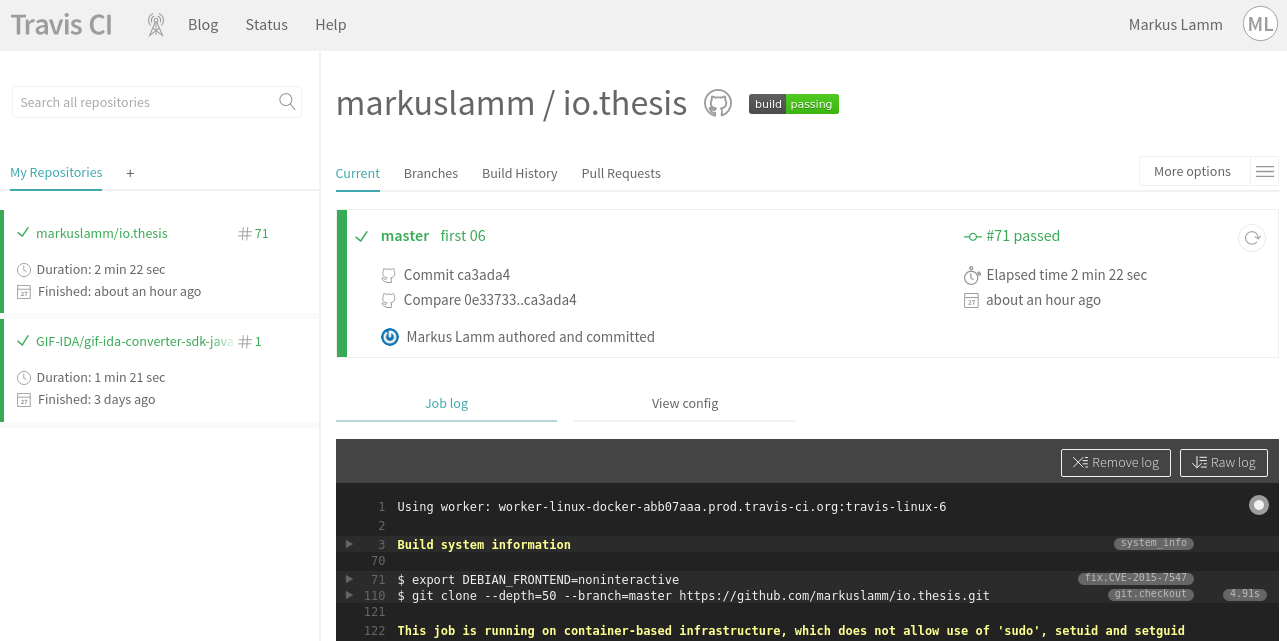
\includegraphics[width=1.0\textwidth]{../images/07-travis.png}
	\caption{Travis CI}
	\label{fig:travis}
\end{figure}

\section{"Collector-Platform" Cluster}
\label{sec:collector-platform-cluster}

According to the proposed architecture in \autoref{ch:architecture}, \textit{"Collector-Platform" Cluster} consists of the
mandatory infrastructure components \textit{Kafka Message-Broker}, \textit{Consul Client-Registry}, \textit{Logstash-Processor} and
\textit{Elasticserach} to fulfill the requirements discussed in \autoref{ch:requirements}. In addition, one instance of
Apache Flink's Job- and TaskManager each will be required, to create a basic Flink cluster acting as data source for the collecting client,
as well as the \textit{Collector-Manager} component for managing the distributed \textit{CollectorClient} instances.

One main challenge of the technical realization of the system solution was to create a cluster of application nodes operating in an
own network distinguishable by their IP addresses. The \textit{"Collector-Platform"} uses Docker to achieve this goal.
Docker provides a "software containerization platform" that allows to wrap applications in a complete filesystem that contains everything
needed to run in form of a container. This container provides an isolated platform for applications to run on Docker host systems
and contains an unix operation system and all required software components required by the application.
Docker uses the resource isolation features of the Linux kernel such as cgroups and kernel namespaces and allow independent containers
to run within a single host instance, avoiding the overhead of starting and maintaining virtual machines.

The applications to be "containerized" will be defined in by a Dockerfile that defines the intructions to build the application container.
The Docker file contains the the behavior of the application when it is started by the \verb|docker-engine|. The following
example shows the definition for the \textit{CollectorManager} component:

\begin{lstlisting}[caption={Dockerfile "CollectorManager"}, captionpos=b, label={lst:dockerfile}]
FROM anapsix/alpine-java
MAINTAINER markus.lamm@googlemail.com
ADD collector-manager-app/target/collector-manager-app.jar /apps/collector-manager-app.jar
ENTRYPOINT ["java","-jar","/apps/collector-manager-app.jar"]
\end{lstlisting}

The resulting container is based on the Docker image \verb|anapsix/alpine-java| which provides an unix operating system and a Java
installation as a base system, the \textit{CollectorManager} will be installed on. In line 3, the \verb|collector-manager-app.jar|
will be copied from the local file system to a virtual path inside the Docker container. The last command in line 4 defines the entry point
for the \verb|docker-engine|, this commmand will be executed on container startup, means the \textit{CollectorManager} jar file will
be executed by the JVM provided by the \verb|anapsix/alpine-java| base image.

Based on the required components discussed above the application needs the following Docker containers:

\begin{itemize}
	\item One Apache Kafka container as message broker and source system for data collection. The Kafka container depends on
	another container for Apache Zookeper as a centralized service for configuration and distributed synchronization and is mandatory
	for the Kafka container to work.
	\item One Consul container as client discovery service
	\item Two Apache Flink containers, one Job- and TaskManager as source systems
	\item One container conatining Logstash, Elasticserach and Kibana
	\item One container for the \textit{CollectorManager} component
\end{itemize}

For the orchestration of the container infrastructure, Docker provides a file format that allows the definion of required containers
and their dependencies in a custom \verb|docker-compose.yml| file. The next section covers main configuration details for the containers
of the \textit{"Collector-Platform"} cluster.

\subsection{Configuration}

The Apache Kafka is a core component of the platform and operates as a buffer between the data producing \textit{CollectorClient}s.
The following excerpt from the \verb|docker-compose.yml| file defines the container for Kafka:
\begin{lstlisting}[caption={Container definition Kafka}, captionpos=b, label={lst:docker-kafka}]
  kafka:
    container_name: kafka
    image: wurstmeister/kafka
    ports:
      - "9092:9092"
      - "9997:9999"   # jmx
      - "9097:9091"   # collector-client
    environment:
      KAFKA_ZOOKEEPER_CONNECT: zookeeper:2181
      KAFKA_ADVERTISED_HOST_NAME: 192.168.2.100 //THIS NEEDS TO BE ADJUSTED ON LOCAL EVALUATION
      KAFKA_CREATE_TOPICS: "collector-outbound-topic:1:1,flink-outbound-topic:1:1"
      JMX_PORT: 9999
      SPRING_PROFILES_ACTIVE: kafka-broker-jmx
      SPRING_CLOUD_CONSUL_HOST: consul
      SPRING_CLOUD_CONSUL_PORT: 8500
      CLIENT_PORT: 9091
      KAFKA_BROKER_ADDRESS: kafka:9092
    volumes:
      - /var/run/docker.sock:/var/run/docker.sock
    depends_on:
      - zookeeper
      - consul
\end{lstlisting}

This configuration defines the required information for running this container. It defines the required ports and dependencies to other containers,
\verb|zookeeper| and \verb|consul| in this example. Furhermore it creates a set of environment variables, containing
connection infos for zookeeper and the kafka address, that needs to be adjusted to the local IP address. Due to the fact that
this container will also be a source system for the \textit{CollectorClient}s, the JMX port is specified to allow the client to access
the remote JVM of Apache Kafka. Other variables contain information
required by the \textit{CollectorClient} Spring Boot application, that needs to be copied to the Docker description of Apache Kafka.

\begin{lstlisting}[caption={CollectorManager copy in Apache Kafka conatiner}, captionpos=b, label={lst:docker-copy-client}]
echo "Start collector client for Apache Kafka..."
java -Djava.security.egd=file:/dev/./urandom -jar /usr/local/collector/collector-client-app.jar
\end{lstlisting}

Another configuration for the definition of the container \textit{CollectorManager}, that defines the required port for the managers user
interface, the dependency to the Consul container as well as environment variables required by the Spring Boot application.

\begin{lstlisting}[caption={CollectorManager container configuration}, captionpos=b, label={lst:docker-manager}]
  collector-manager:
    container_name: collector-manager
    image: io.thesis/collector-manager
    ports:
      - "9090:9090"
    depends_on:
      - consul
    environment:
      SERVER_PORT: 9090
      SPRING_CLOUD_CONSUL_HOST: consul
      SPRING_CLOUD_CONSUL_PORT: 8500
\end{lstlisting}

For the complete configuration of the \textit{"Collector-Platform"} cluster, please refer to Appendix A in \autoref{app:docker-config}

The \verb|docker-compose| file format provides a mechanism to build the \textit{"Collector-Platform"} cluster shown in
\autoref{fig:deployment-diagram}:

\begin{figure}[H]
	\centering
	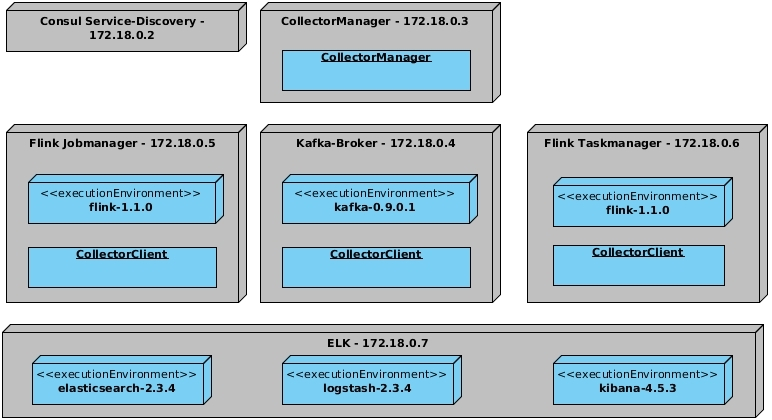
\includegraphics[width=1.0\textwidth]{../uml/deployment-diagram.jpg}
	\caption{Docker Deployment Diagram}
	\label{fig:deployment-diagram}
\end{figure}

To build all required software components and Docker images, and to copy the \verb|collector-client.jar| into the containers of source systems,
the following shell script is used:

\begin{lstlisting}[caption={build-docker-images-sh}, captionpos=b, label={lst:docker-build-images}]
echo "building sources..."
mvn install -DskipTests -DskipITs

echo "cleanup containers..."
docker rm -f $(docker ps -a -q)

echo "building collector-manager-app..."
docker build -t io.thesis/collector-manager collector-manager

echo "building docker-base..."
docker build -t wurstmeister/base infrastructure/docker-base

echo "building docker-zookeeper..."
docker build -t wurstmeister/zookeeper infrastructure/docker-zookeeper

echo "building docker-kafka..."
cp collector-client/collector-client-app/target/collector-client-app.jar infrastructure/docker-kafka/collector-client-app.jar
docker build -t wurstmeister/kafka infrastructure/docker-kafka

echo "building docker-elk..."
docker build -t sebp/elk infrastructure/docker-elk

echo "building docker-flink..."
cp collector-client/collector-client-app/target/collector-client-app.jar infrastructure/docker-flink/collector-client-app.jar
cd infrastructure/docker-flink
./build.sh
\end{lstlisting}

After a successfull building the required software and Docker artefarcts the single command \verb|docker-compose run| starts all
defined containers in the discussed configuration file.

\section{Manual Tests}

The main goal the \textit{Collector-Platform} is to collect system and application data from Apache Flink and Apache Kafka source systems.
Therefore, the system architecture in \autoref{ch:architecture} introduced the \textit{CollectorManager} as the managing component
of distributed \textit{CollectorClient} instances. Hence the \textit{CollectorManager} depends on the Consul Client-Registry,
the Consul container must be up an running. According to the cluster configutation, the Consul container provides a REST endpoint
for listing registered client instances:
\verb|http://localhost:8500|:
\begin{figure}[H]
	\centering
	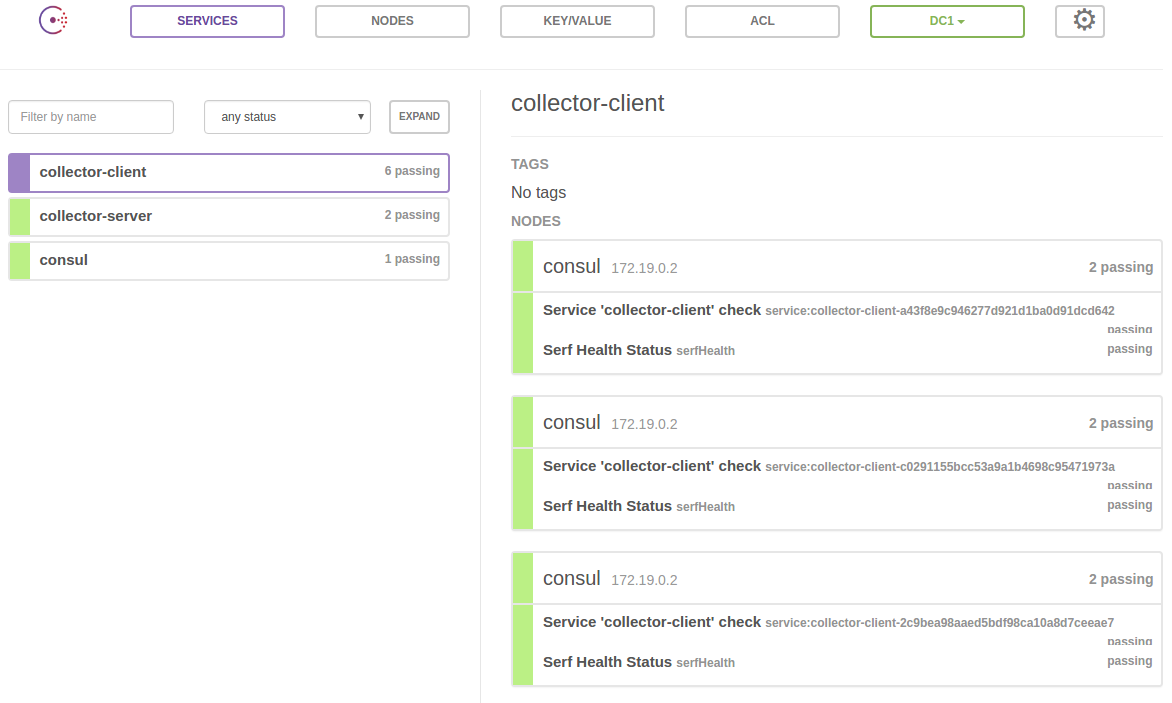
\includegraphics[width=1.0\textwidth]{../images/08-consul.png}
	\caption{Consul web interface}
	\label{fig:consul-web}
\end{figure}

The figure shows three \textit{CollectorClient} instances installed on the \textit{Kafka Message-Broker} as well as the \textit{CollectorClient} instances installed
on the Docker container for Flink's Job- and TaskManager. The presence of the clients in the Consul user interface verifies the
correct functionality of client's self-registrion in the central central registry, that is required to list existing clients in
the user interface with the purpose to schedule the data collection process for individual client instances.

The \textit{CollectorManager} is configured to provide the client listing on \verb|http://localhost:9090|:
\begin{figure}[H]
	\centering
	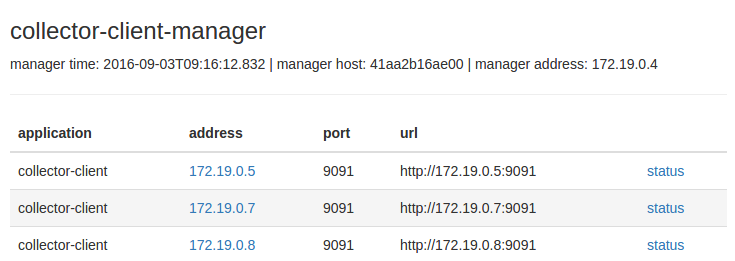
\includegraphics[width=1.0\textwidth]{../images/09-cm-start.png}
	\caption{CollectorManager client listing}
	\label{fig:cm-start}
\end{figure}

In correspondence to \autoref{fig:consul-web}, the \textit{CollectorManager} is able to fetch required client data using the the \textit{Consul Client-Registry}.
This figure shows a very nice feature of Spring Boot, which provides a basic \verb|/health| endpoint for web applications and enables the
\textit{CollectorManager} to link to this endpoint of all \textit{CollectorClient} instances. Because of that, the user interface
of the managing component provides basic monitoring capabilities of registered client instances.

The detailed view of a \textit{CollectorClient} instance provides additinal metadata, fetched from the clients \verb|/client/metadata|

the current
%
%CollectorDataProcessor: module to analyze the data streams creating derived streams and persist flat
%data -> data transformation, analytics layer
%
%Kibana dashboard, show visualization of CollectorDataProcessor data

\section{Discussion}

platform independent of clients, scalable
%Wurden Sie überrascht? Stimmten Ihre Hypothesen? Sind Sie besser, anders als das andere System?
%Wichtigster Erkenntnisgewinn 1
%Wichtigster Erkenntnisgewinn 2
%Wichtigster Erkenntnisgewinn N
%Anwendbarkeit? Szenario?
\section{Summary}

TODO

%Beschreibung  der Ergebnisse, Diagramme, Darstellen von Zusammenhängen